\documentclass{article}
\usepackage{graphicx}
\usepackage{hyperref}

\begin{document}

\title{Project 1}
\author{Jake Carlson}
\date{September 17, 2017}
\maketitle

\abstract
In this report, I will be examining how the United States federal government changed under President George W. Bush and President Barack Obama. I will look into the campaign platforms for each president, determine expectations for how the federal government would resize to meet each president's campaign promises, and then analyze policy decisions made by each president and their effects on the federal payroll. I will also examine natural disasters and geopolitical events that occured during each presidency and how the federal government reacted. We will see that despite Bush's stance on shrinking the government during his campaign, he will end hiring a range of new employees to fill the Department of Homeland Security. We will also see the Obama attracted younger employees to join government work.
\newpage

\tableofcontents
\newpage

\section{Business Understanding}
For this report, I will be examining federal payroll data obtained by BuzzFeed News using the Freedom of Information Act. While the data set itself dates back to 1973, I will only be examining the data relevant to the presdency of George W. Bush (2001 - 2008) and Barack Obama (2009 - 2014). Although Obama's presidency lasted from 2009 to 2016, the data (at the time of writing this report) is only available through to 2014.
\par
Since Bush is a Republican, and Obama a Democrat, we would expect a dichotomy in their policy decisions. Generally, Republican candidates run a campaign focused on shrinking the federal government and lowering taxes, while Democratic candidates tend to emphasize coordination with allies and government solutions to domestic problems. These are common trends for each party, but presidential candidates know that winning the presidency means winning party leadership, so each candidate will support changes in policy that draw new voters and reform their respective parties.

    \subsection{Political Careers}
    Each president had to build up a strong political career before they were considered by their parties as viable presidential candidates. Both presidents's early lives and careers are summarized below.

        \subsubsection{George W. Bush}
        George W. Bush was born in New Haven, Connecticut on July 6, 1946. His family moved to Odessa, Texas in 1948, and then to Midland, Texas in 1950. Bush began elementary school in Midland and finished in Houston after the family moved there in 1959. Bush went to high school at Phillips Academy Andover in Andover, Massachusetts where he developed a love for American History. He went to college at Yale University where he majored in history with a concentration in European and American studies. After he graduated in 1968, he joined the National Guard. He then continued his education at Harvard University where he obtained his MBA. George Bush met Laura Welch in July 1977 and they were married on November 5, 1977. Their twin girls were born in November 1981.\cite{bushhistory}
        \par
        Bush began his political career by campaigning to be the Mayor of Odessa when he was 31. He lost the election, but was on the campaign trail soon after to assist his father's run for the presidency in 1988. He then assisted in his father's reelection campaign in 1982, but they were defeated by Bill Clinton. Bush returned to Texas where he decided to run for Governor. He focused his campaign on education, juvenile justice, and welfare policies. He won the campaign, and worked hard with Texas Democrats to follow through with his campaign promises. His most notable legislative accomplishment was overhauling the Texas education system, adding more choice and competition to the system and setting new skill requirements for children. He also introduced tax cuts, programs to help faith-based organizations, and began providing social services through churches.\cite{bushhistory}
        \par
        He won reelection as governor in 1998 and coined the term "compassionate conservatism", a brand meant to unite Republican values of the free market and small government with social welfare. His success as governor made him a prime choice to run for the presidency in the eyes of the Republican party.\cite{bushhistory}

        \subsubsection{Barack Obama}
        Barack H. Obama II was bown in Hawaii on August 4, 1961. His parents divorced and, after his mother remarried, he moved to Indonesia with his mother and stepfather. His mother was concerned about his education so she sent him back to Hawaii to live with his grandparents. He attended Punahou School from fifth grade through the end of high school. He then went to college, first at Occidental in Los Angeles, and then at Columbia University in New York City. He majored in political science and graduated in 1983. Obama then moved to Chicago to work as a community organizer. He organized the citizens of Altgeld Gardens to pressure Chicago's city hall to improve the living conditions in the public housing project. Unsatisfied with his success, he resolved to get a law degree. He attended Harvard Law School in 1988 and graduated magna cum laude. He met Michelle Robinson shortly after graduation and they were married in 1992. They had two daughters born in 1998 and 2001.\cite{obamahistory}
        \par
        Obama first ran for a political office in 1996, when he ran to be a state senator in Illinois. Despite being a member of the minority party in the state legislature, he was able to work with Republicans and Democrats to pass campaign finance reform and crime legislation. He became a leading legislator after the Democrats won Senate majority and passed nearly 300 bills focusing on helping children, elderly, labor unions, and the poor. He then set his sights on a 2004 race for a U.S. Senate seat. He differentiated himself by opposing Bush's war in Iraq. He won the Senate seat by the largest margin in the history of Senate elections in Illinois.\cite{obamahistory}
        \par
        Obama's stance against the war set him apart from other potential Democratic presidential candidates. In a keynote address he gave at the Democratic National Convention in 2004, he struck notes of unity between political parties and different ethnicities. He promoted optimism with a phrase he borrowed from Reverend Jeremiah Wright, "the audacity of hope".\cite{obamahistory}

    \subsection{The Bush Presidency}
    Every presidency starts out with a campaign for office. A successful candidate makes a number of promises over the course of the campaign in hopes of getting voted into power. It is important that candidates tailor their policies to their constituents, so they don't drive away the coalition that votes their party into positions of power. The campaign is also an opportunity for candidates to present a vision for the future of their party. In the campaign that won Bush the presidency, some of the political policies we would expect to see to accomplish these promises and some of the major events that occured during his presidency that altered how he governed.

        \subsubsection{The 2000 Presidential Campaign}
        The 2000 presidential campaign was a time to reform the Republican party. After the Clinton presidency, the Republican party wanted to move away from unpopular positions such as opposition to all government programs. Bush wanted a party that worked to improve education, expand health care, and increase funding for Social Security and Medicare. He wanted the party to calm their rhetoric on morial issues such as abortion. Bush also spoke about cutting taxes for all Americans, while Democratic candidate Al Gore proposed tax cuts only as part of broader plans to implement policy. The two candidates also differed on how to combat teen pregnancy. Democrats wanted to implement sex education programs in public schools, while Republicans depended on teaching abstinence to teenagers.\cite{bushcampaign2000}
        \par
        Bush denied that climate change was a major issue. Having made a substantial profit when Bush Exploration merged with Spectrum 7 in 1984, he had a vested interest in denying climate change and made it part of his campaign platform.\cite{bushhistory}
        \par
        With these campaign promises, we would expect several areas of the government to get an increase in funding. The Department of Education should see an increase in funding to implement Bush's proposed education program, and the Department of Health and Human services should see an increase in funding to expand health care. However, if Bush implements his tax cuts, we should see funding cuts for a variety of other agencies to offset the loss in revenue the government pulls in. One such organization could be the Internal Revenue Service. We could also see cuts to the EPA in an effort to curb government support for researching climate change.

        \subsubsection{The Presidency}
        Bush wins the Electoral College in 2000 despite falling short of achieving a majority of the popular vote. This leads Democrats to contest the result of the election, calling for recounts in several contested Florida counties. By the end of 2000, the Supreme Court voted to stop the recounts, and Gore conceded, leaving Bush President-elect.
        \par
        After his inauguration in January, 2001, Bush is quick to reinstate a ban on providing aid to organizations that perform abortions. He then moves to abandon the ratification of the Kyoto Protocol, which charged 180 countries to set limits on industrial emissions. In June, Bush signs a \$1.35 trillion tax cut into law that reduces taxes for all income brackets and moves to eliminate the estate tax. Bush also outlines a new policy on stem cell research, where funding is continued for existing research, but bans the collection of additional stem cells.\cite{bushevents} It is typical for first-month presidents to begin enforcing policies that were not enforced by the previous leadership. This gives the appearance that they are enthusiatically getting to work to deliver on campaign promises.
        \par
        On September 11, 2001, the United States is attacked by members of the extremist group Al Qaeda. These individuals hijacked four airplanes and crashed two into the World Trade Center and one into the Pentagon. The fourth was suspected to be headed for the White House, but the passengers fought back againsts the hijackers and diverted the plane off course. It is the deadliest attack on American soil since the Japanese attacked Pearl Harbor. In an address to the nation, Bush vows to bring the group responsible to justice. With in the month, Bush appoints Pennsylvania governor Tom Ridge to a cabinet-level position to oversee the Office of Homeland Security. Ridge is tasked with coordinating efforts across over fourty federal agencies to protect the United States against future terrorist attacks.\cite{bushevents}
        \par
        Trailing his education reform in Texas as governor, in early 2002, Bush signs into law an education reform bill reinstating the No Child Left Behind policy. The bill provides more flexibility to local authorities on how they allocate funds and requires new standardized tests for math and reading.\cite{bushevents}
        \par
        Bush's National Security Advisor, Condoleezza Rice, is questioned by Congress for information about warning signs before September 11th. In response, Bush announces sweeping changes to the security departments, placing the Office of Homeland Security in charge of over 100 agencies responsible for protecting the United States.\cite{bushevents} This marks a change in domestic policy that will likely result in additional funding for various security departments. The pressure to make this change originated from Congress, meaning the group responsible for the budget also supports this consolidation of power.
        \par
        Despite the ongoing war in Iraq, Bush continues to sign tax cuts into law, signing the third largest tax cut in history into law in May, 2003. In June of 2005, the Senate passes an energy bill meant to support the oil and natural gass energy industries, while providing tax incentives for the use of alternative energy sources. July of 2005 sees the launch of space shuttle Discovery, the first launch since the space shuttle Columbia failed during atmospheric reentry in 2003.\cite{bushevents}
        \par
        In August of 2005, Hurricane Katrina ravaged the Gulf coast and severely damaged the city of New Orleans. The levee systems meant to protect the city from flooding failed, causing massive destruction. Rather than allocating FEMA funds to the disaster, the White House is mute on the issue. The administration is harshly criticized for failing to use emergency funds to support aid the city.
        \par
        Bush approves a 700 mile long fence along the U.S.-Mexico border on October 26, 2006. We expect to see a spike in funding for Customs and Border Security around this time.
        \par
        The DOW Jones industrial average begins a sharp decline after an all-time high of 14,164 on October 9, 2007. As the housing crisis begins to set in, Bush proposes a stimulus package to encourage individuals to spend money and stimulate the slowing economy. The Senate votes to pass a slightly smaller stimulus package a few months later, providing Americans with tax rebates and businesses with tax breaks. The federal government resorts to taking over Fannie Mae and Freddie Mac in September, 2008 in an attempt to protect more than half of the country's mortgages. Bush then signs in a \$700 billion bailout plan to protect failing bank assets, the largest in history. He follows up with a bailout of General Motors and Chrysler to keep the two auto manufacturers afloat shortly before leaving office. \cite{bushevents}

    \subsection{The Obama Presidency}
    Obama's run for the presidency started in a tough fought race for the Democratic nomination. He was able to beat out the other top contender, Hillary Clinton, because of his opposition to the war, and his tone of change that he used through out the campaign. Hillary's key theme was experience, but as the economy deteriorated under Bush, Democratic voters favored Obama's platform and gave him the nomination. Obama saw his oportunity to reshape the Democratic party.

        \subsubsection{The 2008 Presidential Campaign}
        On the night of the Democratic National Convention, Obama outlined what he wanted to get done in office. Some of his main promises were cutting taxes for 95\% of tax paying families, end the dependence on foreign oil while investing in renewables, and providing affordable health care to all Americans. He reiterated his desire to end the war in Iraq and expressed that he wanted to close the corporate loopholes that halted the growth of the economy.\cite{obamacampaign2008}
        \par
        The housing market really began to tumble during the presidential debates. Obama was able to win over voters with his calm demeanor and confidence. Republican nominee John McCain began to loose his lead. Obama was able to outspend McCain on campaign advertising, and his vice presidential nominee, Joe Biden, had strong foreign policy experience as the chairman of the Senate Committee on Foreign Relations. This contrasted McCain's running mate, Sarah Palin, who showed little experience with domestic or foreign policy issues.\cite{obamacampaign2008}
        \par
        Obama won the Electoral College by a margin of 365 to 173, with 53\% of the popular vote. He was able to win back key states from the Republicans, like Virgina, Florida, North Carolina, and Ohio.

        \subsubsection{The Presidency}
        The young president was quick to issue an executive order to close Guantanamo Bay. Similar to Bush, he was trying to deliver early on a campaign promise to close the controversial prison. However, he was unsuccessful and the prison still remains open.
        \par
        Obama also got to work right away trying to combat the financial crisis. He required companies receiving federal bailout money to cap executive pay to \$500,000 a year. He also signed the American Recovery and Reinvestment Act to provide relief to those most affected by the crisis.\cite{obamaevents}
        \par
        In February of his first year, Obama also pulled back Bush restrictions on how much money could go to stem cell research. He followed this in October by lifting a ban that prevented people with HIV and AIDS from entering the United States. He closed October by signing The Matthew Shepard and James Byrd Jr. Hate Crimes Prevention Act to help local authorities investigate hate crimes and prosecute perpetrators more effectively.\cite{obamaevents} Around this time, we expect to see an increase in payroll for the Department of Justice as they implement new invesitgation tactics.
        \par
        In early 2010, Obama announces \$900 million in grants for schools that are underperforming. He follows this with the signing of the Affordable Care Act, the implementation and regulation of which will likely increase the number of employees required by the Department of Health and Human Services.
        \par
        In March, Obama announces that he will allow exporatory drilling for oil and gas in the Gulf of Mexico and in the Atlantic Ocean off the coast of Virginia. Drilling in these areas had previously been banned, but he allowed drilling in an attempt to reduce dependency on foreign oil, one of his campign promises. Unfortunately, in April of 2010, the Deepwater Horizon oil rig explodes, killing 11 workers. BP was leasing the oil rig, and signed off on continuing drilling before a pressure seal had been completely tested. The company again endangers the ecosystem of the Gulf of Mexico when a massive oil spill happens in June. Obama says the company will have to pay heavy reparations for their neglect.\cite{obamaevents} It will be interesting to see which agencies, if any, add employees to help manage the crisis in the Gulf and prevent similar events from happening again.
        \par
        In April of 2010, Obama proposes increasing the NASA budget by \$6 billion over the next five years. He wants to see the money used for space exploration over lunar exploration.\cite{obamaevents}
        \par
        Obama takes a stab at veteran education reform with a post-911 GI Bill, mean to assist veterans of the U.S. military in recieving cheap or free college tuition.\cite{obamaevents} Efforts to implement this will likely require additional employees at the Veterans Affairs and the Department of Education.
        \par
        In the end of 2010, Obama institutes a two-year pay raise freeze for federal employees. This is meant to help curb the deficit, and will definetly impact the federal payroll starting in 2011. However, this is followed by the Healthy, Hunger-Free Kids Act which allocates money for funding nutrition education and free lunch programs at public schools.
        \par
        As Obama entered his second term, he put immigration reform and climate change in the spotlight. He outlined a plan for comprehensive immigration reform just after his first week of being reelected. He followed a few months later with the Climate Action Plan, which was meant to lower carbon polution and prepare the country for the pending effects of climate change. He made it clear that reversing climate change is a task for the whole planet.\cite{obamaevents} As Obama steps up his fight against cliamte change, we would expect the EPA to receive additional funding for cliamte science. It will also be interesting to see how Customs and Border Protection responed to his immigration reform.

    \subsection{Congress}
    Just because a president allocates money for a program, doesn't mean the payroll for the agency responsible will be affected. Congress is ultimately responsible for managing the budget of the U.S. government. This means that the party in control of the House of Representatives and the Senate has more control over the budget than the president. If the president leads the party that controls either the House or the Senate, they will likely be able to implement more of their policies. However, if the president's party is the minority party in either of the chambers, they will meet more opposition as they try to push policy. Table \ref{tab:1} shows the party in control of each chamber of Congress.
    \par
    Based on the majority party in each chamber of Congress, Bush should have faced minimal opposition for his first term and the first half of his second term. Obama entered office with a Democratic House and Senate. He should have been able to move policy most effectively during the first half of his first term. It will be interesting to see how his policy was effected by Republicans gaining back the House during his first term.

        \begin{center}
            \begin{table}
                \centering
                \begin{tabular}{ |c|c|c|c| }
                    \hline
                    \multicolumn{4}{|c|}{Majority Party} \\
                    \hline
                    Year & President & Senate & House \\
                    \hline
                    2001 & Bush & Republican & Republican \\
                    2003 & Bush & Republican & Republican \\
                    2005 & Bush & Republican & Republican \\
                    2007 & Bush & Democratic & Democratic \\
                    2009 & Obama & Democratic & Democratic \\
                    2011 & Obama & Democratic & Republican \\
                    2013 & Obama & Democratic & Republican \\
                    2015 & Obama & Republican & Republican \\
                    \hline
                \end{tabular}
                \caption{Party in Control of the House and the Senate}
                \label{tab:1}
            \end{table}
        \end{center}

\section{Data Understanding}
The federal payroll data was obtained through the Freedom of Information Act by BuzzFeed News. For this report I will be examining the status files, which contain payroll information for each agency organized by quarter. I will not be examining accessions or separations in this report.
\par
The status files contain relevant attributes needed for a payroll system such as employee name, the agency they work, their age, education level, length of service, and pay. Each entry also contains a PseudoID which can be used to identify an individual employee. I will further describe each attribute below. These definitions were created using the FedScope Data Definitions document and translation files included with the data set.\cite{datadefs}

    \subsection{PseudoID}
    A unique identifier for an employee. This value is sufficient for identifying an employee in a table. If a table contains duplicate PseudoIDs, an employee must of either been transfered to another organization, or had their pay change.

    \subsection{Name}
    The name of the employee if it is provided by the agency. Some employee names have been withheld by the agency they work for. These entries have "Name Withheld by Agency" in place of the name. The name of an employee is not useful for understanding how the federal government changes under a president, so this attribute will not be used.

    \subsection{Date}
    The date the pay report is generated up to. Because the tables are quarterly, the date for each quarter will be the same for all entries. This is the last day in March, June, September, and December.

    \subsection{Agency}
    This is a categorical variable representing the department the employee worked at. The departments are encoded as six characters. The first four characters represent the top level organization the department belongs to. The last two characters are unique to the department for identification. The provided file "SCTFILE.txt" can be used to translate between the agency encoding and the actual name of the agency.
    \par
    For example, the Food and Drug Administration is encoded as 'AGHE36'. Here, AGHE refers to the Department of Health and Human Services. The value '36' is then used to identify the FDA specifically. All agency entries begin with 'AG' or 'AH', so these characters can be discarded.

    \subsection{Station}
    Station is a categorical variable that refers to the actual location the employee worked at. This is encoded in a 9 character string. The first two characters represent the state the employee worked, characters 3-6 map to a city, and characters 7-9 encode a county.

    \subsection{Age}
    This is an ordinal attribute that holds the age of the employee. Ages are broken down into the age ranges of five years starting with 15-19, 20-24, and going up to 70-74 and then 75+.

    \subsection{Education}
    Education is another ordinal attribute that encodes the level of education the employee achieved. This is represented as a two digit number that maps to a description of the education level. Examples are 04 for High School Graduate, 13 for a Bachelor's Degree, 17 for a Master's Degree, and 21 for a Doctorate Degree.

    \subsection{PayPlan}
    Pay plan is a two character categorical variable loosely representing the type of work the employee does. This is used by the governemnt to determine the rate of pay increases. Some examples are 'EE' for expert, 'EG' for consultant, and 'EX' for executive.

    \subsection{Grade}
    Grade is a categorical variable used in conjunction with PayPlan to determine an employees basic pay rate.

    \subsection{LOS}
    LOS is an ordinal variable representing the length of service in years of the employee. Length of service is grouped by the following time spans: < 1, 1-2, 3-4, 5-9, 10-19, 20-24, 25-29, 30-34, and 35+.

    \subsection{Occupation}
    Occupation is a categorical variable classifying workers as blue or white collar. The value can be more desciptive by looking into occupation families, but the data attribute category also encodes this information so I will not be using this field.

    \subsection{Category}
    Category is a categorical variable representing the type of work the employee does. It is a single character in the PATCO acronym which follows the translation in Table \ref{tab:2}.

        \begin{center}
            \begin{table}
                \centering
                \begin{tabular}{ |c|c| }
                    \hline
                    Letter & Translation \\
                    \hline
                    P & Professional \\
                    A & Administrative \\
                    T & Technical \\
                    C & Clerical \\
                    O & Other White Collar \\
                    B & Blue Collar \\
                    \hline
                \end{tabular}
                \caption{PATCO Translation}
                \label{tab:2}
            \end{table}
        \end{center}

    \subsection{Pay}
    Pay is a ratio representing the annual pay of the employee in U.S. dollars.

    \subsection{SupervisoryStatus}
    A categorical variable representing what level of leadership the employee is at. This follows the translaton in Table \ref{tab:3}.
    \par
    Here, CSRA refers to a private organization that provides IT solutions to the federal government.

        \begin{center}
            \begin{table}
                \centering
                \begin{tabular}{ |c|c| }
                    \hline
                    Status Code & Translation \\
                    \hline
                    2 & Supervisor or Manager \\
                    4 & Supervisor (CSRA) \\
                    5 & Management Official (CSRA) \\
                    6 & Leader \\
                    7 & Team Leader \\
                    8 & All Other Positions \\
                    \hline
                \end{tabular}
                \caption{Supervisory Status Translation}
                \label{tab:3}
            \end{table}
        \end{center}

    \subsection{Appointment}
    Appointment is a categorical variable representing if the position is expected to be permanent, nonpermanent, career, or career-conditional.

    \subsection{Schedule}
    A categorical variable describing if a position is full-time, part-time, intermittent, or seasonal.

    \subsection{NSFTP}
    Another categorical variable representing if a position representing is a position is seasonal for full-time, permanent employees. NSFTP can be translated using Table \ref{tab:4}.

        \begin{center}
            \begin{table}
                \centering
                \begin{tabular}{ |c|c| }
                    \hline
                    NSFTP Code & Translation \\
                    \hline
                    1 & Non-seasonal, Full-time, Permanent \\
                    2 & Seasonal, Full-time, Permanent \\
                    \hline
                \end{tabular}
                \caption{NSFTP Code Translation}
                \label{tab:4}
            \end{table}
        \end{center}

\section{Data Preparation}
The data comes in text files with fixed width columns. Dr. Hahsler provided us with some initial code to read in one of the text files, break up the attributes into columns, apply a header to the columns, remove common characters from the Agency column, and create a new column called AgencyName with the translation from the four character Agency identifier to the full agency name. This is was a good starting point, however, there is more to be done before the data is clean enough to begin analysis. After my cleaning pipeline was functional, I wrote R code to apply the pipeline to every status file in the data set. I grouped cleaned data frames by year and saved each year to its own CSV file for quick reloading as I moved into data modeling.

    \subsection{Agency Subsetting}
    The first thing I do is throw out agencies that I don't want to examine. Based on my business understanding, I selected agencies that were specifically mentioned as receiving attention by each president at some point in their two terms. I also selected agencies that I thought would show differences in the political affiliations and leadership policies of the two presidents. I perform this subsetting as the first stage in my pipeline to reduce the amount of data that has to flow through the rest of the pipeline. The agencies I chose are listed in Table \ref{tab:5}.

        \begin{center}
            \begin{table}
                \centering
                \begin{tabular}{ |c|c| }
                    \hline
                    Agency & Agency Code \\
                    \hline
                    Department of Health and Human Sevices & AGHE, AHHE \\
                    Department of Homeland Security & AGHS, AHHS \\
                    Department of Housing and Urban Development & AGHU, AHHU \\
                    Department of Energy & AGDN, AHDN \\
                    Department of Education & AGED, AHED \\
                    Department of Justice & AGDJ, AHDJ \\
                    Department of the Interior & AGIN, AHIN \\
                    Department of Transportation & AGTD, AHTD \\
                    Environmental Protection Agency & AGEP, AHEP \\
                    Federal Emergency Management Agency & AGEM, AHEM \\
                    General Services & AGGS, AHGS \\
                    NASA & AGNN, AHNN \\
                    National Security Agency & AGSP, AHSP \\
                    Internal Revenue Service & AGTR07, AGTR93 \\
                    Veterans Affairs & AGVA, AHVA \\
                    \hline
                \end{tabular}
                \caption{Agencies Chosen for Analysis}
                \label{tab:5}
            \end{table}
        \end{center}

    \subsection{Unknown Values}
    Many of the entries have values encoding for unknown or missing information in at least one of the attributes. For example, the Age column uses "UNSP" to show that the age of the employee is unspecified. Other values that indicate missing data are a string of asterisks or an empty field. It is necessary to convert these values to NA, which R uses to encode that an attribute is missing for an entity.
    \par
    When R reads in a data file, it assumes all attributes are 'factors', or categorical variables. Many of the attributes are categorical variables, but fields like Age and Education are ordinals. I need to convert these to ordered factors, R's representation for an ordinal, before moving forward. Also, Pay needs to be converted from a factor to a numeric value.

    \subsection{Imputation}
    After converting these field to more accurate data classes, I work to impute some unknown values. Starting with Age, I replace an unknown employee Age with the median Age for employees at the same Agency. I thought this was a good method for imputing Age because if some agencies have outliers in Age, either very young or very old, the median will not be dramatically affected by these values like the mean would.
    \par
    I then impute Education by taking the median Education level achieved by employees of the same Age at that Agency. The majority of employees in the federal government achieved a Bachelor's degree, so this was a common value that was used to fill in unknown Education.
    \par
    Finally, I impute Pay using the median Pay for employees of the same Age at the Agency. This is a good method because the annual pay for an employee at any organization is closely related to their work experience, which can be loosely approximated based on their age. This will also separate based on Agency, so that if some Agencies receive higher Pay on average, the imputed value more closely represent the separation.
    \par
    After imputation, I throw out any entries where Pay could not be imputed. If the Agency an employee worked at was not known, the above imputation method would not return a value. Without knowing the Pay or the Agency an employee worked at, the amount of useful information that can be gathered is severely reduced, so these entries are removed.

    \subsection{Duplicates}
    Next, I handle duplicate PseudoIDs. As stated earlier, a PseudoID will occur multiple times if an employee changed agencies during the quarter or if their pay changed. If an employee changed organization, I will want to include their salary when determining the total value of the payroll for each of those organizations, so these entries will be left as is. However, if an employee simply received a raise while working at the same organization, I want to remove the lower of the salaries. This makes the assumption that the employee earned that same ammont during the whole quarter, but since we are looking at payroll data with the level of granularity of the quarter year, this is acceptable.

\section{Analysis}
With the data set cleaned, I can now begin analysis. We will start with simple data exploration to find the attributes that are most useful for describing changes to the federal government. I will be examining the years 2001, 2005, 2009, and 2013. These represent are the years of inauguration for each of the presidents's terms, and will, at a high level, show how their policies are changing the government.

    \subsection{Simple Statistics}
    I will skip simple statistics for PseudoID and Date because their values are used only for identification of individuals and time.

        \subsubsection{Station}
        Let's look at the states with the most federal employment in the years chosen above. I will use substring to grab the first two characters in the Station column. I map this to the state name using a translation table provided in the data set. Then I count the occurences of the states and sort the entries in descending order. The result can be seen in Table \ref{tab:6}.
        \par
        I expected the most populated states to have the most employees. It also makes sense that DC would have the most employees, being the center of the government. It is interesing how Florida gradually overtakes Pennsylvania and New York in the number of employees. Next I will provide the average number of employees in each state for each of these years. This will do a good job showing how the overall size of the govenrment changes over the course of this timespan. The averages can be seen in Table \ref{tab:7}.
        \par
        Interestingly, we see the largest increase in the average number of federal employees between the beginning of Bush's second term and the inauguration of Obama, despite the Republican's support for a smaller government. Also, Obama grows the government more in his first term than Bush did in his first term. I will have to explore these numbers more to see which agencies specifically were recieving additional employees.

            \begin{center}
                \begin{table}
                    \centering
                    \begin{tabular}{ |c|c|c|c|c|c|c|c|c| }
                        \hline
                        year & 2001 & 2005 & 2009 & 2013 \\
                        \hline
                        rank & State | Count & State | Count & State | Count & State | Count \\
                        \hline
                        1 & DC | 195,701 & DC | 207,993 & DC | 231,997 & DC | 246,609 \\
                        2 & California | 163,895 & California | 170,589 & California | 188,056 & California | 199,593 \\
                        3 & Maryland | 156,112 & Maryland | 165,670 & Maryland | 177,874 & Maryland | 196,400 \\
                        4 & Texas | 129,741 & Texas | 136,488 & Texas | 157,398 & Texas | 168,109 \\
                        5 & New York | 114,721 & New York | 110,724 & Florida | 120,900 & Florida | 130,690 \\
                        6 & Pennsylvania | 82,909 & Florida | 101,691 & New York | 117,739 & New York | 119,592 \\
                        \hline
                    \end{tabular}
                    \caption{States with the Highest Number of Employees}
                    \label{tab:6}
                \end{table}
            \end{center}

            \begin{center}
                \begin{table}
                    \centering
                    \begin{tabular}{ |c|c|c| }
                        \hline
                        Year & Average Employees \\
                        \hline
                        2001 & 41828.24 \\
                        2005 & 43895.55 \\
                        2008 & 49347.78 \\
                        2013 & 52324.04 \\
                        \hline
                    \end{tabular}
                    \caption{Average Number of Employees in each State}
                    \label{tab:7}
                \end{table}
            \end{center}

        \subsubsection{Age}
        The most common employee ages for each of the presidents's terms can be seen in Table \ref{tab:8}.
        \par
        The most common age increases slightly under Bush. This is representative of an aging population of employees.

            \begin{center}
                \begin{table}
                    \centering
                    \begin{tabular}{ |c|c| }
                        \hline
                        Year & Mode \\
                        \hline
                        2001 & 45-49 \\
                        2005 & 50-54 \\
                        2009 & 50-54 \\
                        2013 & 50-54 \\
                        \hline
                    \end{tabular}
                    \caption{Most Common Age Intervals by Year}
                    \label{tab:8}
                \end{table}
            \end{center}

        \subsubsection{Education}
        There are 22 education levels employees can fall under. I will look at the three most common education levels for each of my years, and the number fo employees in each category. The results are in Table \ref{tab:9}.

            \begin{center}
                \begin{table}
                    \centering
                    \begin{tabular}{ |c|c|c| }
                        \hline
                        Year & Education Level & Count \\
                        \hline
                        & Bachelor's Degree & 691,023 \\
                        2001 & High School Graduate & 582,996 \\
                        & Master's Degree & 254,444 \\
                        \hline
                        & Bachelor's Degree & 812,014 \\
                        2005 & High School Graduate & 809,430 \\
                        & Master's Degree & 312,071 \\
                        \hline
                        & Bachelor's Degree & 950,459 \\
                        2009 & High School Graduate & 837,441 \\
                        & Master's Degree & 400,777 \\
                        \hline
                        & Bachelor's Degree & 1,033,993 \\
                        2013 & High School Graduate & 839,401 \\
                        & Master's Degree & 499,255 \\
                        \hline
                    \end{tabular}
                    \caption{Employees at the Most Common Education Levels by Year}
                    \label{tab:9}
                \end{table}
            \end{center}

        \subsubsection{LOS}
        To determine what the most common length of service is, I will take the mode of LOS for my four years. The results can be seen in Table \ref{tab:10}.
        \par
        What is interesting here is the sudden decrease in the most common length of service after Obama is inaugurated. The most common LOS increased from 10-14 to 15-19 in Bush's first term. Either the more seasoned employees decided to leave their jobs in objection to some of Bush's policies, or they wanted to exit when Bush's presidency ended. I will have to look at the years between 2005 and 2009 in order to get a better idea of how seniored employees left as Bush's presidency came to a close.

            \begin{center}
                \begin{table}
                    \centering
                    \begin{tabular}{ |c|c| }
                        \hline
                        Year & LOS \\
                        \hline
                        2001 & 10-14 \\
                        2005 & 15-19 \\
                        2009 & 5-9 \\
                        2013 & 5-9 \\
                        \hline
                    \end{tabular}
                    \caption{Most Common Length of Service}
                    \label{tab:10}
                \end{table}
            \end{center}

        \subsubsection{Pay}
        In this section we will look at the mean, median, and max pay for each of the four years. These values are recorded in Table \ref{tab:11}.
        \par
        We can see that the average pay increases across all of the years we analyzed. The average pay jumps \$9,800 from 2001-2005, \$10,100 from 2005-2009, and \$5,000 from 2009-2013. It is interesting that the lowest pay increases occured under Obama, but it makes sense as Obama was trying to get spending under control and combat the financial crisis.
        \par
        Another interesting point is that the max pay increased from \$200,000 when Bush took office to \$401,589 when Obama was inaugurated the second time. Because all of the means are greater than the medians, these large max pays are outliers pulling up the average.

            \begin{center}
                \begin{table}
                    \centering
                    \begin{tabular}{ |c|c|c|c| }
                        \hline
                        Year & Mean & Median & Max \\
                        \hline
                        2001 & \$54,079 & \$48,649 & \$200,000 \\
                        2005 & \$63,872 & \$57,168 & \$250,000 \\
                        2009 & \$73,890 & \$64,961 & \$393,411 \\
                        2013 & \$79,207 & \$72,722 & \$401,589 \\
                        \hline
                    \end{tabular}
                    \caption{Mean, Median, and Max Pay by Year}
                    \label{tab:11}
                \end{table}
            \end{center}

        \subsubsection{SupervisoryStatus}
        I will take the mode of SupervisoryStatus to find what most employees are classified as. The results are in Table \ref{tab:12}.
        \par
        The most common employee is categorized as "Other", meaning they are not a supervisor. The second most common position is "Supervisor or Manager". I will take the ratio of these to see approximately how many employees report to one supervisor.
        \par
        Interestingly, the approximate number of employees reporting to a supervisor consistently shrunk over this timespan. This could mean that supervisors are expected to pick up more responsibilities when they reach supervisor status.

            \begin{center}
                \begin{table}
                    \centering
                    \begin{tabular}{ |c|c| }
                        \hline
                        Year & Mode \\
                        \hline
                        2001 & Other \\
                        2005 & Other \\
                        2009 & Other \\
                        2013 & Other \\
                        \hline
                    \end{tabular}
                    \caption{Most Common SupervisoryStatus Classification by Year}
                    \label{tab:12}
                \end{table}
            \end{center}

            \begin{center}
                \begin{table}
                    \centering
                    \begin{tabular}{ |c|c| }
                        \hline
                        Year & Ratio Other to Supervisor \\
                        \hline
                        2001 & 8.1 \\
                        2005 & 7.7 \\
                        2009 & 7.6 \\
                        2013 & 7.1 \\
                        \hline
                    \end{tabular}
                    \caption{Ratio of Other Type Employees to Supervisors by Year}
                    \label{tab:12}
                \end{table}
            \end{center}


    \subsection{Data Visualization}
    It is important to start data visualization with the creation of histograms so that a better understanding of the underlying distribution of data can be visualized before trying to determine relationships in the data. In this section I will generate histograms for the following attributes: Agency, Age, Education, LOS, and Pay.

        \subsubsection{Agency}
        Figure \ref{simpleagency} shows some interesting trends. First and most notable is the creation of the Department of Homeland Security (HS) by Bush following 9/11. The agency does not show up in 2001, but is the second largest of my choosen agencies by 2005. Also, the size of the agency increases under President Obama. Another agency that grows under Obama is the Office of Veterans Affairs (VA). This is likely in response to the post-911 GI Bill signed by Obama in 2010.
        \par
        Some agencies see a decrease in size between the two presidents. Notably, the IRS (TR) saw decreases in staffing durring each interval analyzed. Bush began the downsizing in the agency following his tax cuts, but the downsizing continued under Obama.

        \subsubsection{Age}
        I will now look at histograms for the number of employees in each age interval for my selected years. See Figure \ref{agehistograms}. With the four plots, we can watch as employees age. Namely, we see employees aged 50-54 entering the 55-59 interval between years 2001 and 2005. We can also see a hiring surge of younger employees in Obama's first term as a negative slant in the 2013 box plot. Lastly, we can see that older employees are choosing to retire at later ages by the increase in size of the bars for the age intervals 60-64, 65-69, and 70-74.
        \par
        An interesting relationship to explore will be how the age of the employee relates to length of service and pay. I would expect a positive correlation between these attributes, as employees who have more experience, or who have worked at an agency for longer, should be paid more.

        \subsubsection{Education}
        Figure \ref{eduhistograms} shows the distribution of education levels for all four of my selected years. As outlined in the simple statistics for Education, the distribution is dominated by employees who have either received a Bachelor's Degree or a High School diploma. In Bush's first term, there is an influx of high school educated employees entering the workforce. However, once Bush leaves office, the number of high school graduates remains fairly constant while the number of employees with Bachelor's and Master's degrees increases under Obama. All other education levels remain fairly constant through out the timespan.
        \par
        In the Relationships section, I want to examine which agencies are recieving the majority of the college and graduate school graduates under the Obama administration.

        \subsubsection{LOS}
        We can see the distribution of length of service for the selected years in Figure \ref{loshistograms}. We can see the mode of the length of service move backward as described in the simple statistics section. Another interesing feature is the surge in employees with less than five years of services between the years 2001 and 2005. This is likely the result of the creation of the Department of Homeland Security by Bush after 9/11. This triggered a hiring surge to fill a variety of new positions meant to defend the United States against terrorism. This relationship will be explored further in the Relationships section.

        \subsubsection{Pay}
        Figure \ref{paydensities} shows the distribution of pay for each of the selected years. The distributions remain fairly consistent. The distribution for 2001 has a strong positive slant. The slant gradualy becomes more neutral as time progresses. The most common pays are typically around \$30,000. The long tail trailing out shows the how the maximum pay changes across each of the years.
        \par
        Another interesting feature that emerges in the 2013 plot is another peak pay around \$80,000. This likely has to do with the addition of employees with Bachelor's and Master's degrees under the Obama administration.

    \subsection{Relationships}

        \subsubsection{Length of Service versus Age}
        Figure \ref{losage} shows length of service plotted against age. The size of the boxes show the quantity of people who fit into each category. We can see from the large box at the bottom of the 15-19 column that there are a lot of young employees who have < 1 or 1-2 years of experience as expected. There is a large block of employees in the age range 40-44 who have 15-19 years of service. The graph shows that there is a strong positive correlation between age and length of service.
        \par
        This trend is consistent over time for employees age 50 and above. However, under the Obama administration, we see more employees between the ages 35-44 who have shorter lengths of service than in the Bush time frame. This indicates a wave of new people joining governemtn work and is consistent with the changing slant of the distribution of ages of employees for 2013 in Figure \ref{agehistograms}.

        \subsubsection{Pay versus Age}
        Figure \ref{payage} shows the distribution of pay for each of the age ranges. I expected pay to increase with age. However, this trend only hold till around age 40. At this point, the mean pay for each subsequent age range is consistent. There is a slight spreading out of the interquartile range, showing that older employees do continue to receive pay increases, but these raises are not applied to the age category as a whole which seems to be  the trend for employees under the age of 40.
        \par
        The most notable change going into 2013 is that the scale of the pay axis changes to represent the large range of pay that is introduced under the Obama administration.

        \subsubsection{Pay versus Station}
        Some states are more expensive to live in. I would expect states like California and New York to have a higher average pay than states in the Mid West. Figure \ref{paystate} shows that California, Texas, Colorado, and Washington have higher pay on average than states in the Great Plains. The darkening of the graph from 2005 to 2013 also shows the general increase in pay that government employees saw over this timeline. Washington DC and Maryland saw the most notable increase in average pay.

        \subsubsection{Pay versus Education}
        Figure \ref{edupay} shows that pay increases with education. There is a noticable cahnge in the pattern where the level of education is First Professional. These individuals have a higher pay on average than all other levels of education. In 2005, there is a wide distribution of pay for individuals with no formal education. It is interesting that this year has such a dramatic separation from all other years chosen in this respect. The range of pay for employees with no formal education decreases under Obama.

        \subsubsection{Pay versus Supervisory Status}
        I used Spearman's correlation to determine if there is a relationship between supervisory status and pay. Spearman's returned a p-value of 2.2e-16 for both 2005 and 2013. This indicates that we can disprove the null hypothesis. There is a relationship between the two values. This is likely a negative correlation indicating that as supervisory status goes from high to low values, the pay goes up. This is because supervisory status is loosely ordered where 2 is supervisor and 8 is other.

\section{Conclusion}
Based off of my analysis, the presidents were consistent with their campaign promises during their terms in office. However, there were some events that triggered changes in policy. The September 11th attacks pushed Bush to create a new department in the federal government to protect the United States. This opened up hiring and resulted in an increase in federal employment. I would have liked to explore changes to FEMA around Hurricane Katrina, but the organization was dropped from by data in preprocessing after the first year was complete.
\par
Obama entered office in the middle of a financial crisis. It was up to him to reshape the government and implement policy to revive the struggling economy. It was interesting seeing the distribution pay increase as Obama's leadership progressed, despite an effort to subvert the financial crisis. If I could examine additional organizations, I would like to look at how the Securities and Exchange Commission changed as Obama's presidency progressed. I would expect to see the regulatory agency increase in size under Obama.
\par
If I had more time, I would like to see what the distribution of education was at each of my selected agencies. I was not expecting to see the IRS decrease in size under the Obama administration. It is possible there were hiring more experienced people to automate some of the most common tasks, resulting in a decrease in the number of employees needed to enforce the tax policy.
\par
I would also expect the Social Security Administration to decrease in size under Bush because he favored privatizing Social Security, and increase under Obama because he favored the opposite. From other students, I have heard that the administration actually increased in size under Bush and shrunk under Obama. I would have liked to explore this relationship more.

\newpage

\begin{center}
    \begin{figure}
        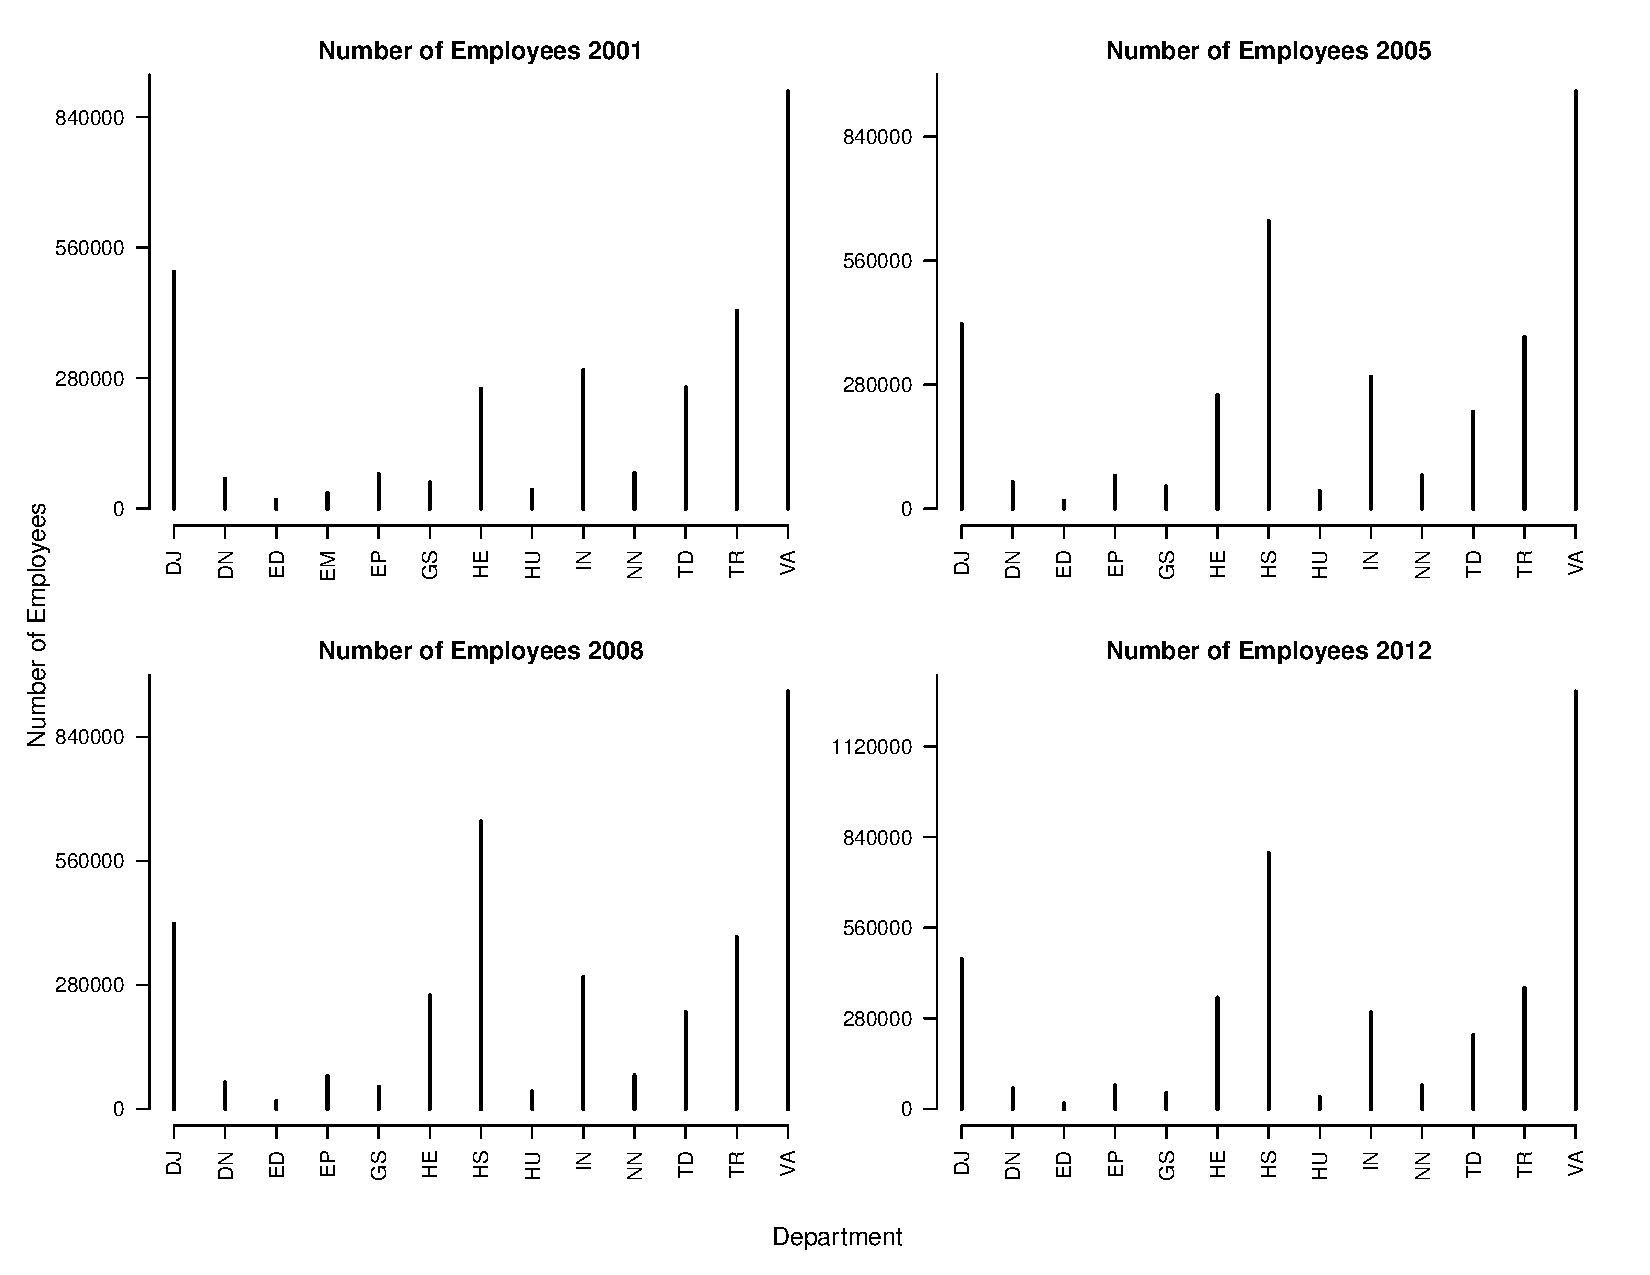
\includegraphics[scale=0.4]{./images/simple-stat-agency.pdf}
        \caption{Number of Employees at Key Departments}
        \label{simpleagency}
    \end{figure}
\end{center}

\begin{center}
    \begin{figure}
        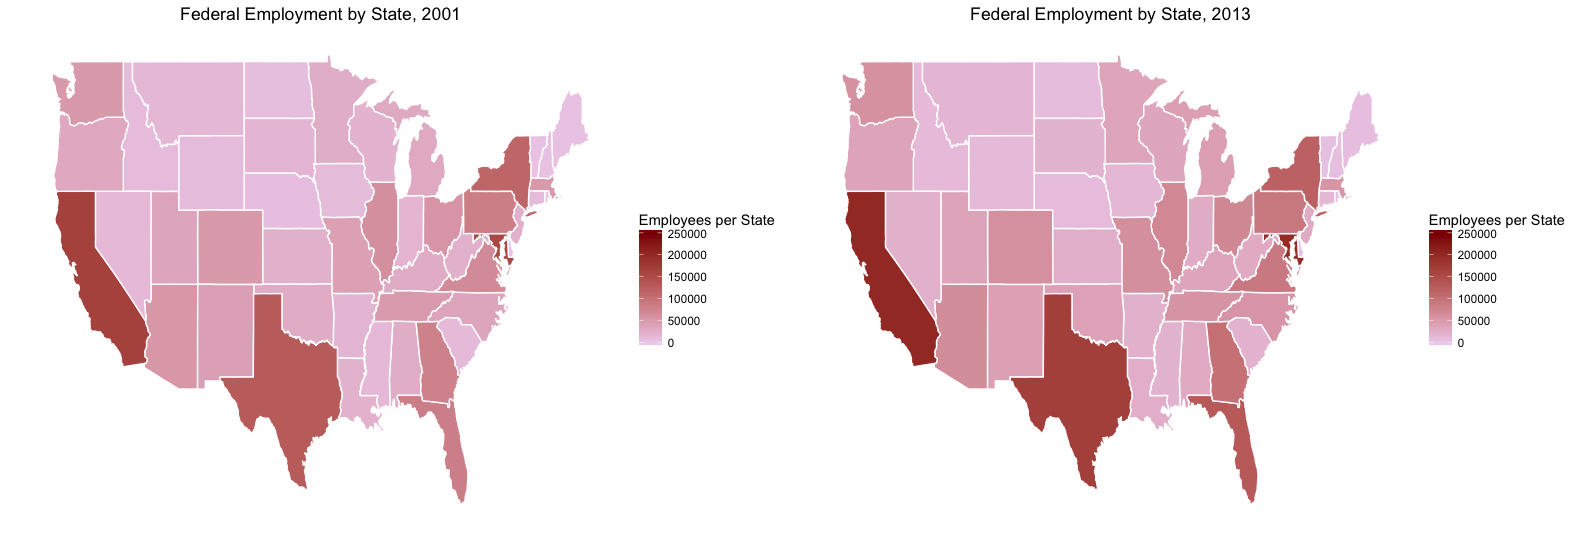
\includegraphics[scale=0.3]{./images/employment-by-state-2001-2013.png}
        \caption{Number of Federal Employees in Continental United States}
        \label{employmentheatmap}
    \end{figure}
\end{center}

\begin{center}
    \begin{figure}
        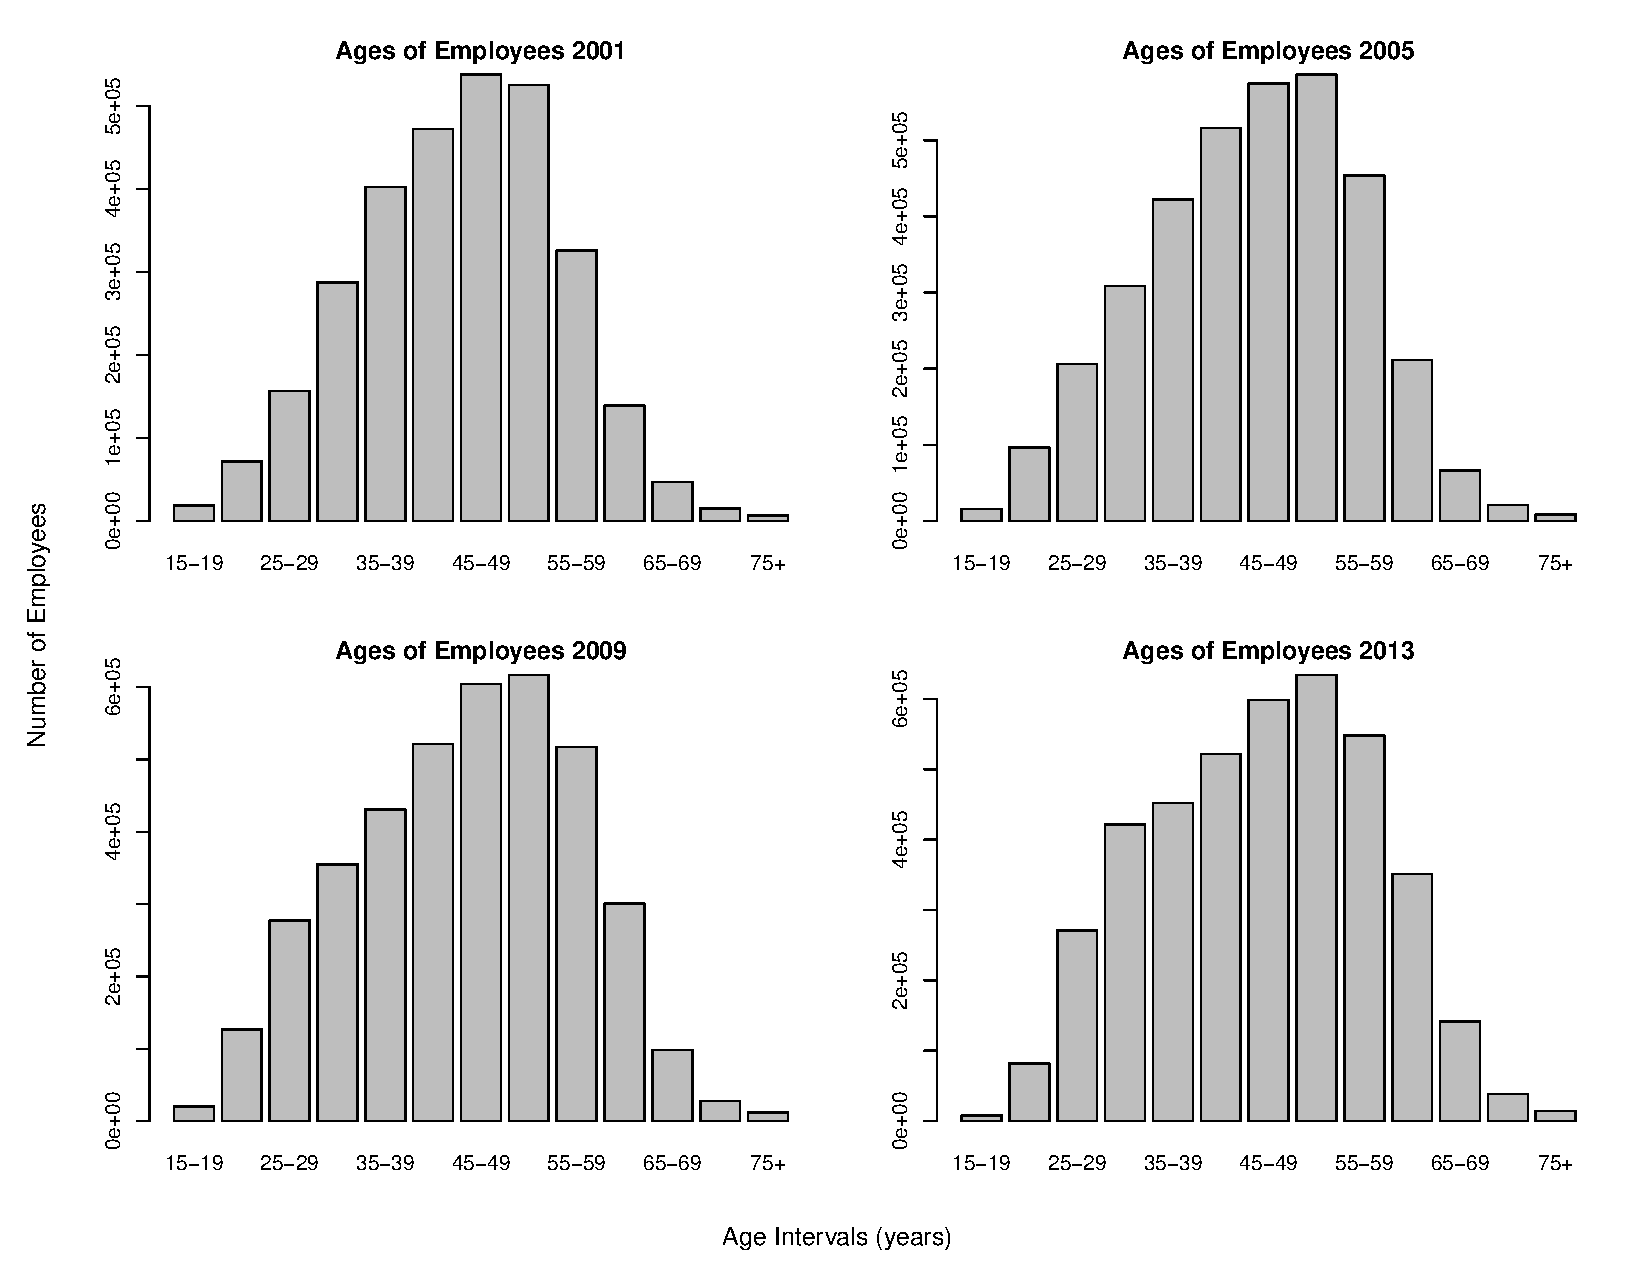
\includegraphics[scale=0.4]{./images/histogram-ages-2001-2013.pdf}
        \caption{Number of Employees in each Age Interval}
        \label{agehistograms}
    \end{figure}
\end{center}

\begin{center}
    \begin{figure}
        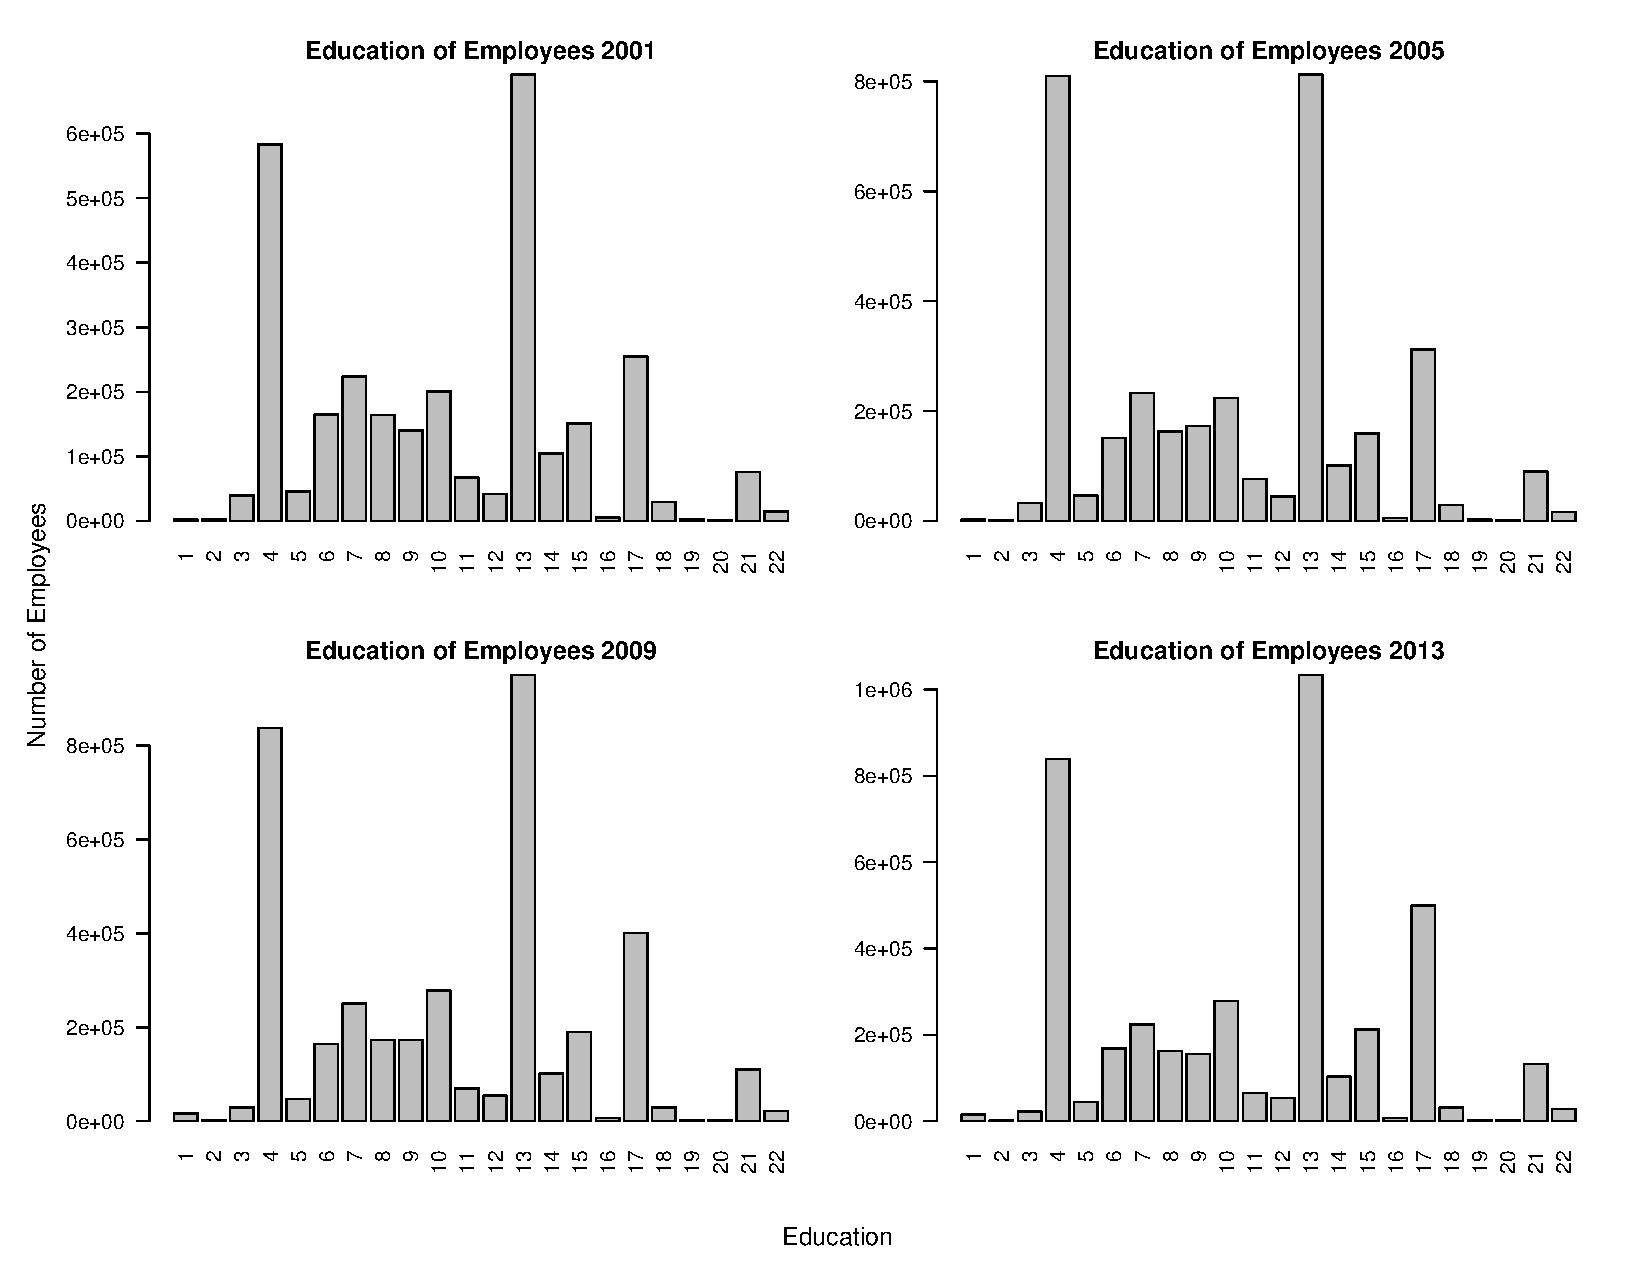
\includegraphics[scale=0.4]{./images/education-histograms.pdf}
        \caption{Number of Employees at Each Education Level by Year, translations in Table \ref{tab:13}}
        \label{eduhistograms}
    \end{figure}
\end{center}

\begin{center}
    \begin{table}
        \centering
        \begin{tabular}{ |c|c| }
            \hline
            Encoding & Education Level \\
            \hline
            01 & NO FORMAL EDUCATION OR SOME ELEMENTARY SCHOOL \\
            02 & ELEMENTARY SCHOOL COMPLETED \\
            03 & SOME HIGH SCHOOL \\
            04 & HIGH SCHOOL GRADUATE OR CERTIFICATE OF EQUIVALENCY \\
            05 & TERMINAL OCCUPATIONAL PROGRAM - DID NOT COMPLETE \\
            06 & TERMINAL OCCUPATIONAL PROGRAM - DIPLOMA OR EQUIV \\
            07 & SOME COLLEGE - LESS THAN ONE YEAR \\
            08 & ONE YEAR COLLEGE \\
            09 & TWO YEARS COLLEGE \\
            10 & ASSOCIATE DEGREE \\
            11 & THREE YEARS COLLEGE \\
            12 & FOUR YEARS COLLEGE \\
            13 & BACHELOR'S DEGREE \\
            14 & POST-BACHELOR'S \\
            15 & FIRST PROFESSIONAL \\
            16 & POST-FIRST PROFESSIONAL \\
            17 & MASTER'S DEGREE \\
            18 & POST-MASTER'S \\
            19 & SIXTH-YEAR DEGREE \\
            20 & POST-SIXTH YEAR \\
            21 & DOCTORATE DEGREE \\
            22 & POST-DOCTORATE \\
            \hline
        \end{tabular}
        \caption{Education Translation}
        \label{tab:13}
    \end{table}
\end{center}

\begin{center}
    \begin{figure}
        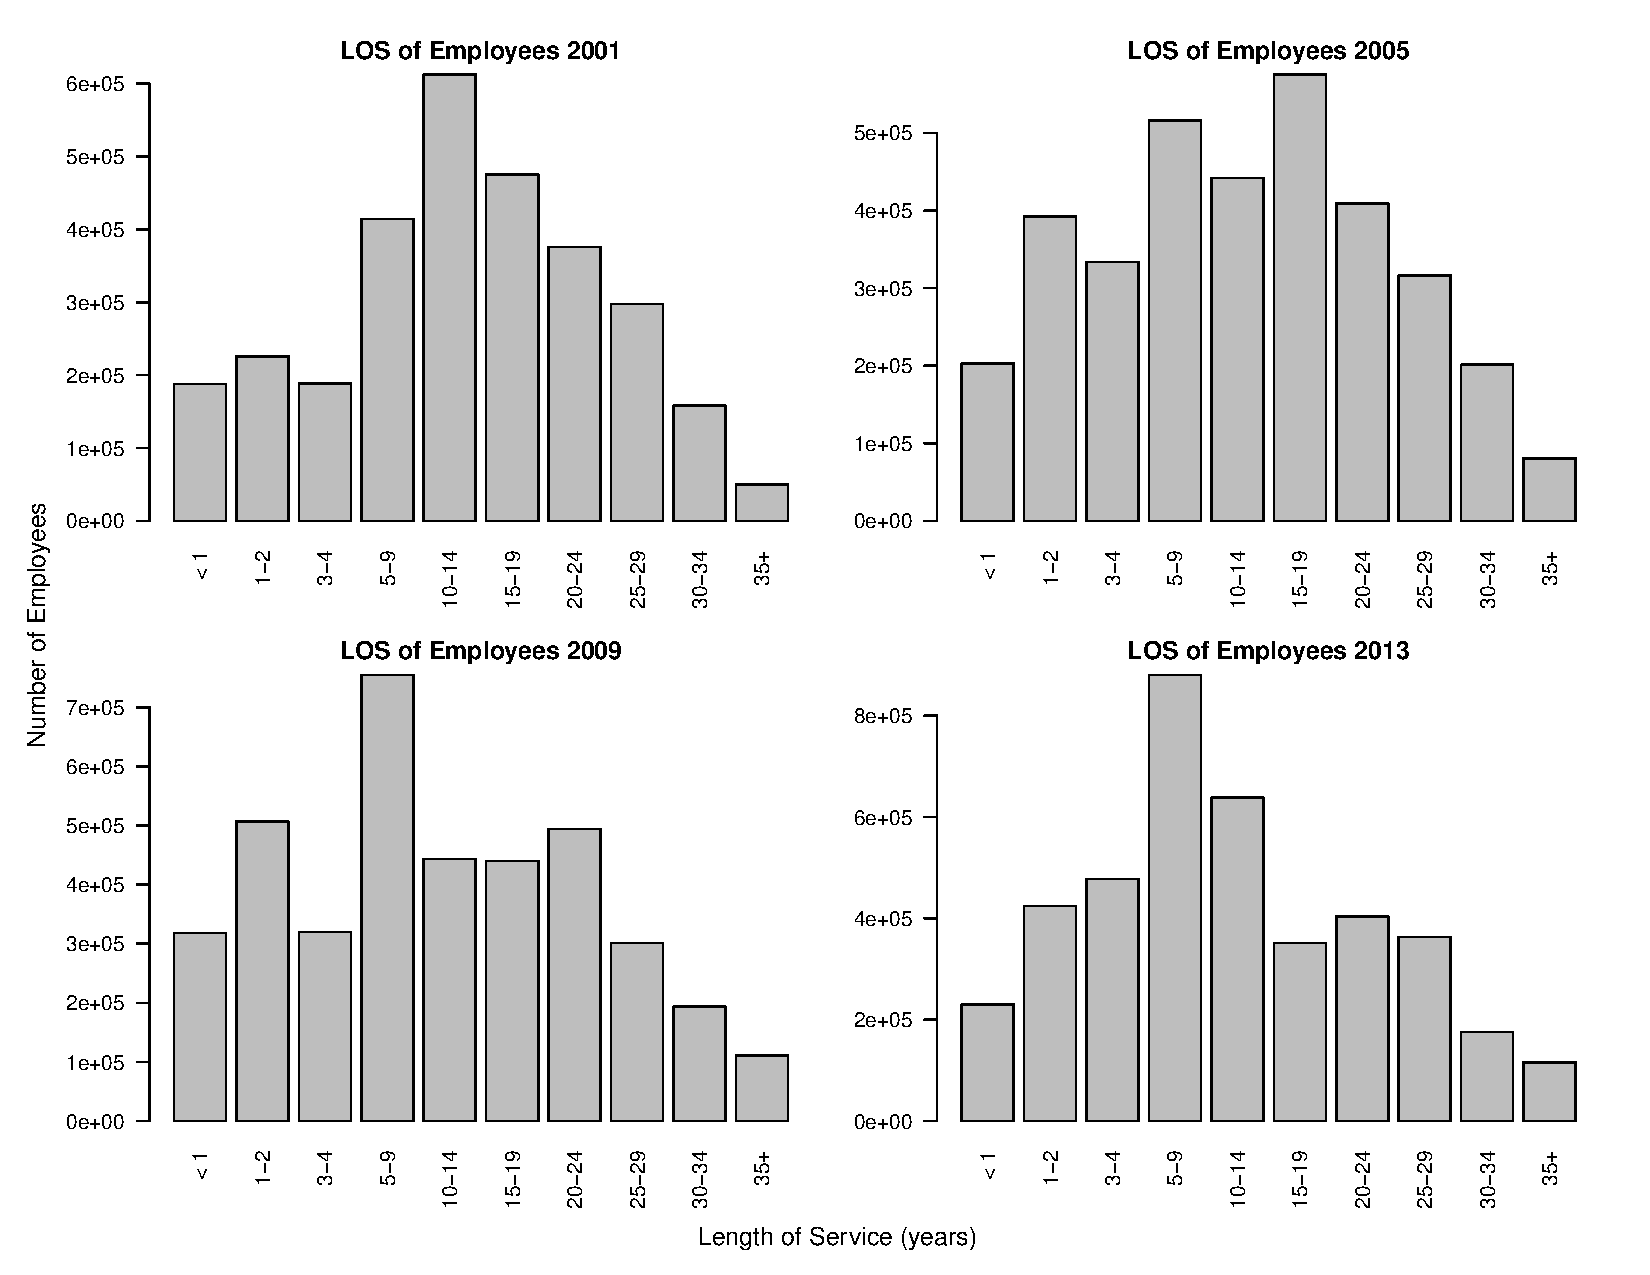
\includegraphics[scale=0.4]{./images/los-histograms.pdf}
        \caption{The Distribution of the Length of Service of Employees for the Selected Years}
        \label{loshistograms}
    \end{figure}
\end{center}

\begin{center}
    \begin{figure}
        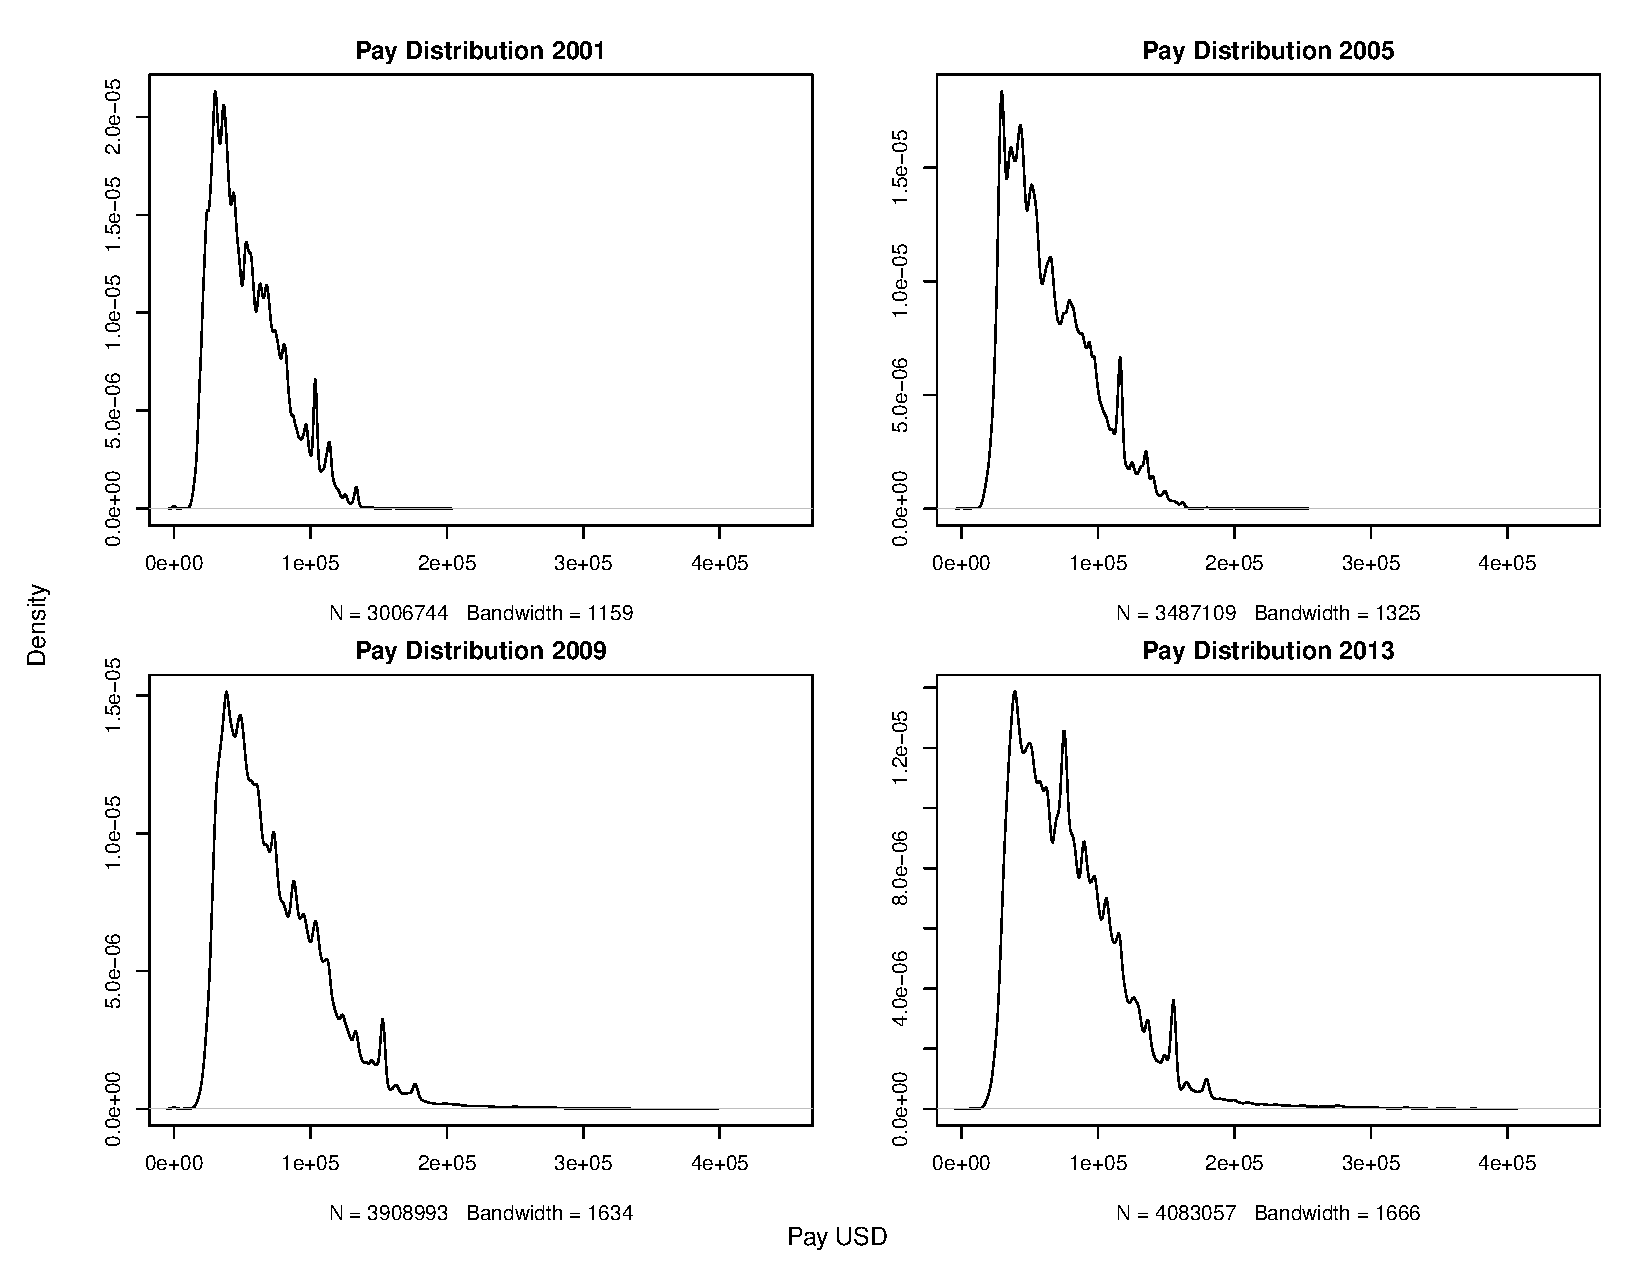
\includegraphics[scale=0.4]{./images/pay-density.pdf}
        \caption{The Pay Density for Each of the Selected Years}
        \label{paydensities}
    \end{figure}
\end{center}

\begin{center}
    \begin{figure}
        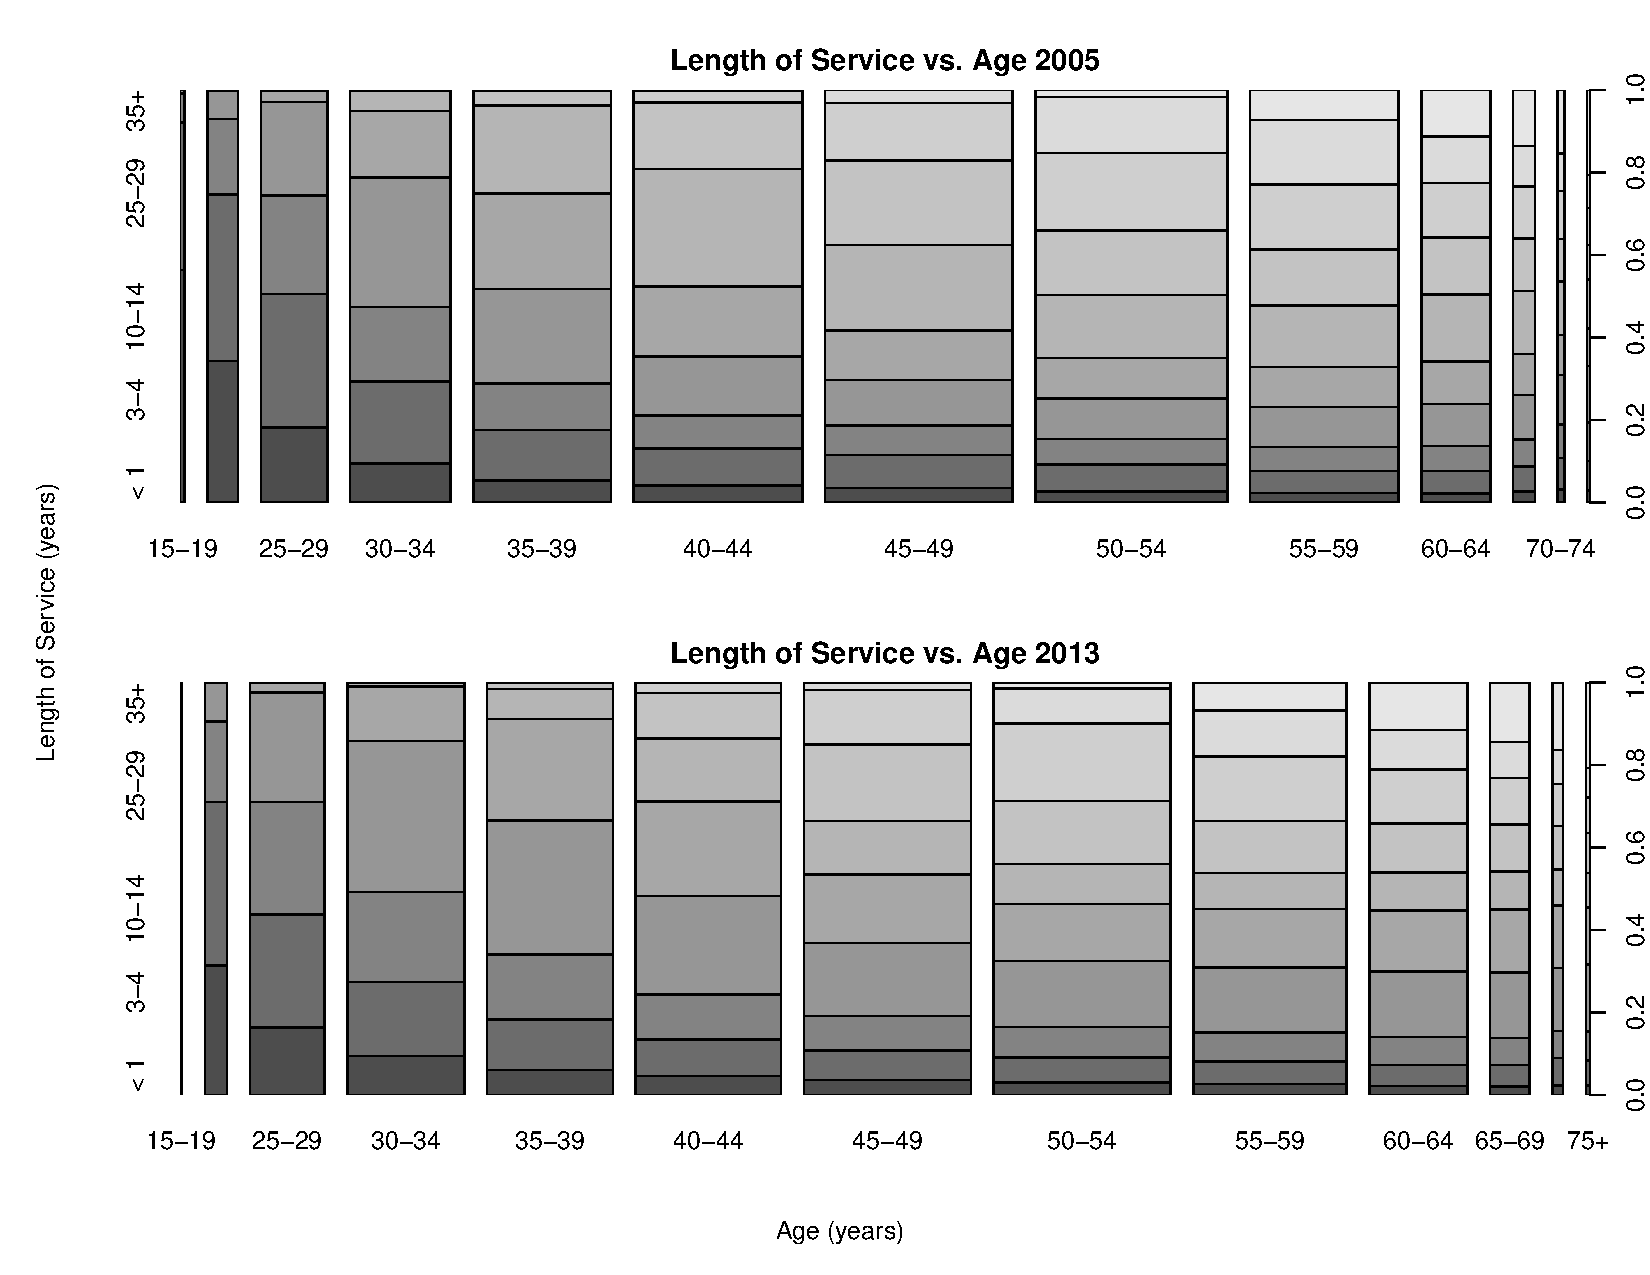
\includegraphics[scale=0.4]{./images/los-age.pdf}
        \caption{Length of Service Plotted Against Age}
        \label{losage}
    \end{figure}
\end{center}

\begin{center}
    \begin{figure}
        \includegraphics[scale=0.4]{./images/pay-age.pdf}
        \caption{Pay Plotted Against Age}
        \label{payage}
    \end{figure}
\end{center}

\begin{center}
    \begin{figure}
        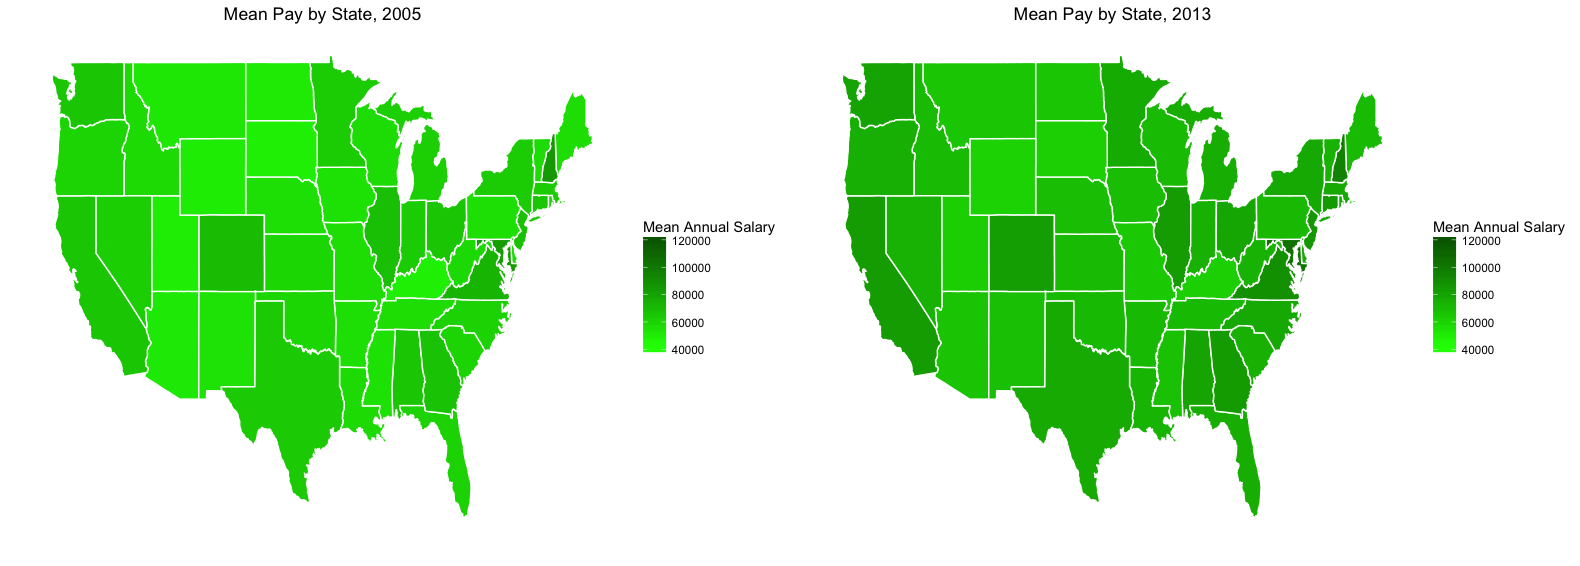
\includegraphics[scale=0.3]{./images/pay-state.png}
        \caption{Average Pay per State}
        \label{paystate}
    \end{figure}
\end{center}

\begin{center}
    \begin{figure}
        \includegraphics[scale=0.4]{./images/edu-pay.pdf}
        \caption{Distribution of Pay by Education, Courtesy of Jenn Le}
        \label{edupay}
    \end{figure}
\end{center}

\newpage

\begin{thebibliography}{10}
    \bibitem{bushhistory}
    Gary L. Gregg II
    \textit{George W. Bush: Life Before the Presidency}
    \texttt{https://millercenter.org/president/gwbush/life-before-the-presidency}

    \bibitem{obamahistory}
    Michael Nelson
    \textit{Barack Obama: Life Before the Presidency}
    \texttt{https://millercenter.org/president/obama/life-before-the-presidency}

    \bibitem{bushcampaign2000}
    Gerald M. Pomper
    \textit{The 2000 Presidential Election: Why Gore Lost}
    \texttt{https://www.uvm.edu/~dguber/POLS125/articles/pomper.htm}

    \bibitem{bushevents}
    University of Virginia - Miller Center
    \textit{George W. Bush - Key Events}
    \texttt{https://millercenter.org/president/george-w-bush/key-events}

    \bibitem{obamacampaign2008}
    Michael Nelson
    \textit{Barack Obama: Campaigns and Elections}
    \texttt{https://millercenter.org/president/obama/campaigns-and-elections}

    \bibitem{obamaevents}
    University of Virginia - Miller Center
    \textit{Barack Obama - Key Events}
    \texttt{https://millercenter.org/president/barack-obama/key-events}

    \bibitem{datadefs}
    United States Office of Personnel Management
    \textit{FedScope Data Definitions}
    \texttt{https://ia800608.us.archive.org/16/items/opm-federal-employment-data/docs/}
    \texttt{FedScope\%20-\%20DataDefinitions}

\end{thebibliography}

\end{document}
